% Created 2014-12-08 Mon 09:48
\documentclass[11pt]{article}
\usepackage[utf8]{inputenc}
\usepackage[T1]{fontenc}
\usepackage{graphicx}
\usepackage{longtable}
\usepackage{float}
\usepackage{wrapfig}
\usepackage{soul}
\usepackage{amssymb}
\usepackage{hyperref}


\title{Optimizer}
\author{miles}
\date{08 December 2014}

\begin{document}

\maketitle

\setcounter{tocdepth}{3}
\tableofcontents
\vspace*{1cm}
\section{Building \& Running}
\label{sec-1}

  Steps to build and run our DAMAJ Decaf Compiler.
  
  These instructions assume you are running on Athena.
  
  Clone the repository or otherwise obtain a copy of the code.

  Run \texttt{add -f scala}. use \texttt{scala -version} to make sure that scala is using version 2.11.2.
  We use \texttt{fsc} to compile scala a little faster. If you happen to have any trouble because of weird
  fsc version conflicts, please try killing your fsc server (find it with \texttt{ps aux | grep fsc}).
  Don't set any env variables like \texttt{SCALA\_HOME} as this could force you to use the wrong version
  of scala.
  
  Once you have the right version of scala run \texttt{make} or \texttt{build.sh} to compile the project.
  If you have trouble with this or later steps, try `make clean` to reset the build files.
  
  Now you should be able to run the compiler using run.sh.

  To enable optimizations you can add \texttt{-O all}.

  For example:

  \texttt{./run.sh --debug tests/codegen/input/01-callout.dcf -O all}

  \texttt{./run.sh --debug tests/codegen/input/04-math2.dcf -o 04-math2.asm}

  Alternatively, you can use \texttt{compile.sh} to compile and run a program.
  \texttt{./compile.sh tests/codegen/input/01-callout.dcf}
  This will assemble the program into \texttt{tmp/out.S}, print the assembly, create an executable at \texttt{tmp/out},
  and run the executable, printing its output as well. This will not work for programs which need to be
  linked to external libraries, for those please use \texttt{run.sh} or another script.
  
\section{Optimizations}
\label{sec-2}

  Some of the optimizations below were previously described in `doc/data$_{\mathrm{flow}}$/DataFlowAnalysis.pdf`.
  They are described here again because many described before were disabled and have since been enabled.
  
  Most optimizations use analyses from `src/scala/dataflow`.

\subsection{Interface}
\label{sec-2.1}


  To run the compiler with optimizations use the flag \texttt{-O all} or \texttt{--opt=all}. This will run all implemented
  optimizations with the order specified in the Order section.
  The availabe optimizations are listed below as well as in the \texttt{optimizations} value in \texttt{src/scala/Compiler.scala}.



\begin{center}
\begin{tabular}{lll}
 Short Name   &  Full Name                         &  Source File                              \\
\hline
 cse          &  Common Subexpression Elimination  &  \texttt{CSE}                             \\
 copyprop     &  Copy Propagation                  &  \texttt{CopyPropagation}                 \\
 deadcode     &  Dead Code Elimination             &  \texttt{DeadCodeElimMulti}               \\
 unreachable  &  Unreachable Code Elimination      &  \texttt{UnreachableCodeElim}             \\
 peep         &  Algebraic Peephole                &  \texttt{PeepholeAlgebra}                 \\
 inline       &  Method Inlining                   &  \texttt{Inline}                          \\
 localize     &  Localization                      &  \texttt{GlobalToLocal}                   \\
 regs         &  Register Allocation               &  \texttt{src/scala/register\_allocation}  \\
\end{tabular}
\end{center}



  Source File in the table to a \texttt{.scala} file in \texttt{src/scala/transform}. There are more transformations
  in that directory that are necessarily utilities but not optimizations.

  Multiple optimizations can also be specified with \texttt{--opt=cse,copyprop} but note that the order listed in the option
  will not have any effect and that the optimizations may be run more than once. If using debug mode, you can tell
  which optimizations were run, how many times, and in what order by looking at stderr or the graph files generated
  in \texttt{tmp/}.

\subsection{Common Subexpression Elimination}
\label{sec-2.2}

    Operates on: Set of Expressions
    Available Expressions Analysis is a forward-running algorithm that determines wether an expressions variables are reassigned before the block. 
    Every assignment to x removes any expressions in the state that depend on variable x 
     
  Here is an example of CSE optimization. Please note that the blocks were given names for debugging 
  purposes, and that circular nodes are forking conditions.

  Before: 

  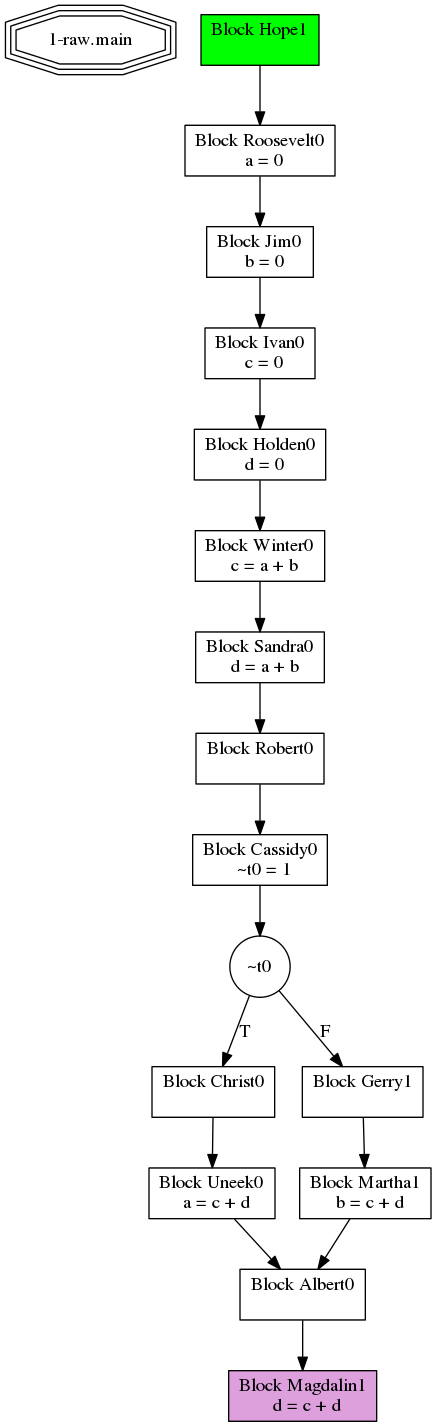
\includegraphics[width=0.4\textwidth]{./before_cse.png}
  
  After CSE:

  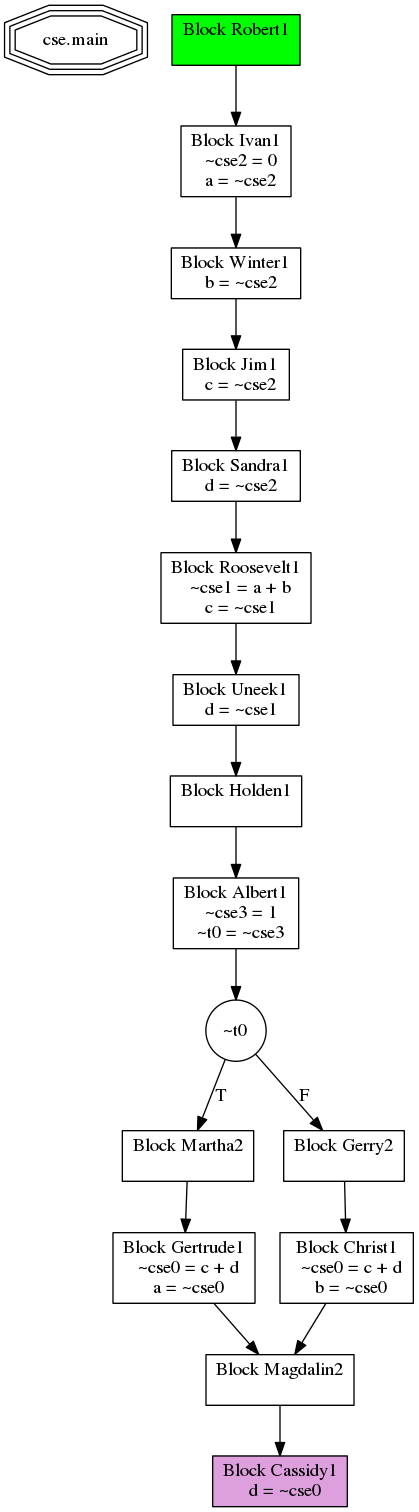
\includegraphics[width=0.4\textwidth]{./after_cse.png}

  Notice that CSE temps are generated for the expressions \texttt{0}, \texttt{a+b}, and \texttt{c+d}, and also that \texttt{c+d}
  appropriately is available for the last statement after it became available in each input branch. 


\subsection{Unreachable Code Elimination}
\label{sec-2.3}

    Unreachable code elimination, located in \texttt{src/scala/transform/UnreachableCodeElim.scala}, 
    deletes portions of code which can never be reached. It consumes the Reachable analysis. Any 
    block code deemed unreachable by Reachable is turned into a nop block with no statements. The 
    nop blocks are cleaned up in a later pass by the Condenser.

    Here is an example of UCE at work. Note that the blocks after the return in the if are not cleared because they could occur, but the blocks after the definitive return are cleared.


\subsection{Dead Code Elimination}
\label{sec-2.4}

  If there is an assignment to a dead variable, it is first checked for whether it is a method call. 
  If it is, it is converted simply to a method call without an assignment. Otherwise, the assignment
  to a dead variable is removed completely. 

  Here is an example of before and after Dead Code Elimination runs. Please note that the blocks were
  given names for debugging purposes, and that circular nodes are forking conditions.

  Before: 

  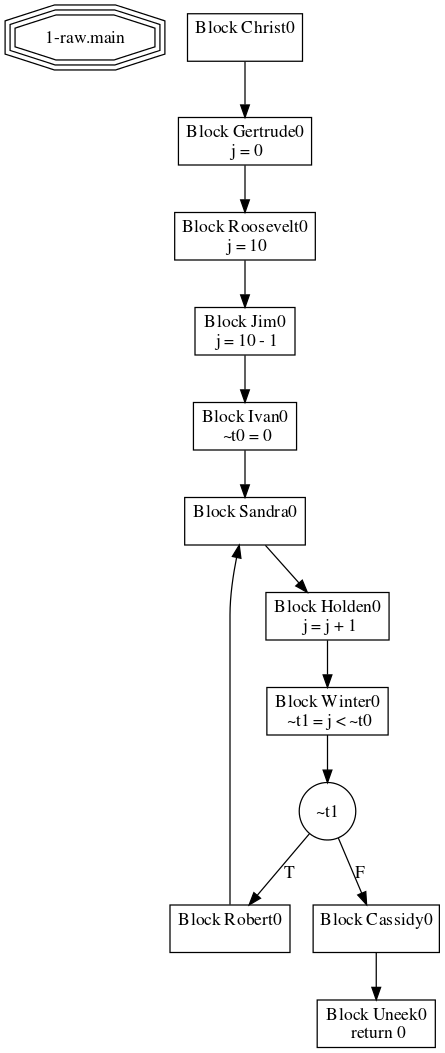
\includegraphics[width=0.4\textwidth]{./before_deadcode_example.png}
  
  After dead code elimination:

  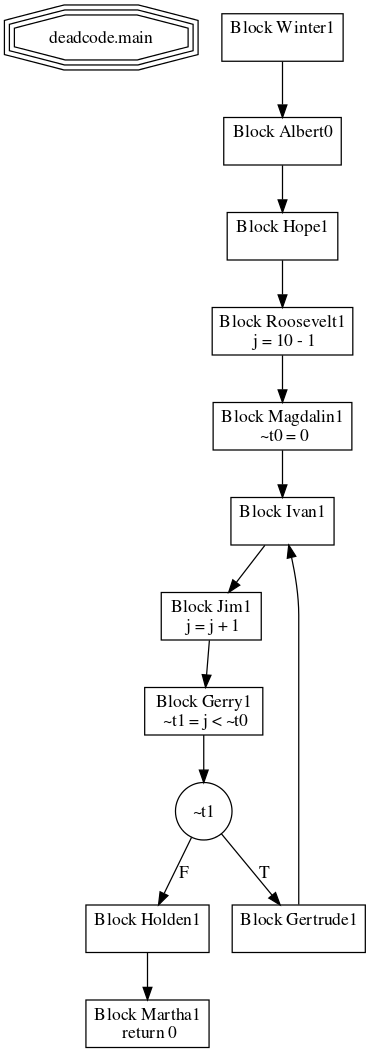
\includegraphics[width=0.4\textwidth]{./after_deadcode_example.png}

  Notice that the dead statements have been removed (the now-empty blocks will be removed in a later step).


\subsection{Copy Propogation}
\label{sec-2.5}

  Copy Propagation uses the analysis of Reaching Definitions. For every use of a variable, it tries to
  replace that with the last value the variable was assigned (along every path to the current line, 
  hence reaching definitions). We have implemented a simple version that doesn't do a replacement if more
  than one path assigned a value, although it could be modified to make sure that each path assigns the same
  value, and then copy propagate. When there is a viable copy propagation (the right hand side of the reaching
  assignment is a single variable or constant), it is not done if the target value is a parameter and the 
  target asignee is a call argument, because we want to explicitly load parameters into local variables when 
  setting up a call. This is the only specially handled edge case.

  We know copy propagation is beneficial and general because it is one we learned in class. Furthermore,
  its main benefit is in causing unnecessary temps to become unused, so they can be deleted.

  As an example, take this sample code from \texttt{tests/optimizer/input/noise\_median.dcf} in the method \texttt{read}. 
  After the simplification steps that generated 13 temp variables, there was some code that looked like
  this:

  \texttt{t0 = rows; ... i = t7; ... t6 = i < t0;}

  After running copy prop, it looked like this:
  
  \texttt{t0 = rows; ... i = t7; ... t6 = t7 < rows;}

  At that point, t0 was not used anywhere and was able to be eliminated.

\subsection{Algebraic Peephole}
\label{sec-2.6}


  Algebraic peephole optimizations are a set of very local optimizations that operate at the statement level.
  Expressions in assignments are compared to a list of known patterns and replaced.
  Assigns in our IR can not contain method calls so this optimization is not at risk eliminating side-effects
  which would violate the semantics of the program for example \texttt{x()*0 -> 0}.
  Algebraic Peephole can simplify the algebraic identities (in both orders where appropriate):
\begin{itemize}
\item \texttt{x*0 -> 0}
\item \texttt{x*1 -> x}
\item \texttt{x/1 -> x}
\item \texttt{x+0 -> x}
\item \texttt{x-0 -> x}
\item \texttt{0/x -> 0}
\end{itemize}
  
  When both operand values are known at compile time, the compiler will replace the expression with the constant result.
  The optimizations preserves the semantics of array out of bound failures and divide by zero errors.
  There may be a bug that causes the compiler to crash if integer overflow occurs during static evaluation. This should be fixed in the next version.


\subsection{Method Inlining}
\label{sec-2.7}


  Method Inlining is an optimization that takes the CFG of a method call and replaces the call with the CFG.
  This enables other optimizations to apply to the CFG that would otherwise have been blocked by the fact
  that the code was in multiple CFGs.
  There is a heuristic of 128 statements that is a maximum for code inlining. Inlining huge methods
  results in intractibly slow compilation speed because of the scale of the combined graph.


\subsection{Global Localization}
\label{sec-2.8}


  Global Localization turns globals into locals.
  The motivation for this optimization is that many of our other optimizations remain conservative
  by not operating on gloabls. This is because globals are harder to reason about due to their
  sharing beyond the scope of the method.

  Global Localization works by examining which globals are used by which methods, identifying
  globals used by only one method, and moving the global into that methods local symbol table.

  Global Localization is not beneficial by itself, but enables other optimizations which avoid
  operating on globals to operate on those variables after they have been localized.
  Global Localization is made more powerful in some cases by Method Inlining, because inlining
  can cause a global that was used by 2 methods to be uesd by only 1 after inlining, thus GL can operate on the global.


\subsection{Register Allocation}
\label{sec-2.9}

  Relevant files: \texttt{src/scala/register\_allocation/*}

  When run without Register Allocation, all variables end up stored on the stack. 
  We add the ability to store varibles in registers instead of the stack. The registers we use are
  rbx, r12, r13, r14, and r15. We save the others for things like moving stack variables in and other
  things. This could be improved by changing \texttt{AsmGen.scala} to better use those registers, and by
  dynamically allocating variables instead of assigning one variable to one register for the length of
  the method.

  Our method of register allocation uses Live Variables analysis. When two variables are live at the same 
  time, they interfere. From this we construct an interference graph of variables. We try to color this graph.

  We used the coloring method from the slides in class. Push all nodes whose degree is less than the number of colors onto a stack.
  When all nodes have degree less than the number of colors, spill a node onto the program stack and eliminate it from the graph.
  Pop the nodes off the stack one by one, assigning colors that do not conflict with their neighbors.

  Any nodes that cannot be colored by this method will be used from the stack, as previously all the variables
  were.

  Our version of register allocation is conservative because it uses only registers that are not used by
  any other part of the program. It moves variables to and from the ``operation registers'' when it does a
  calculation. This is a simplification that makes register allocation more clearly correct, and still faster
  because register accesses are faster than stack accesses.
  When run without Register Allocation, all variables end up stored on the stack.

  Here is an example to demonstrate the effect of register allocation.
  Consider a simple program with no other optimizations in effect.

\begin{verbatim}
int main() {
    int a, b;
    a = 4;
    b = a;
    return 0;
}
\end{verbatim}



  Without register allocation, a part of the compiled assembly results in this code.
  Which has two memory five memory accesses.

\begin{verbatim}
  movq $0, -8(%rbp) # zero a
._node_1_block:
  movq $0, -16(%rbp) # zero b
._node_2_block:
  movq $4, -8(%rbp) # a = 4
._node_3_block:
  movq -8(%rbp), %r11 # use a transfer register
  movq %r11, -16(%rbp) # to move a to b
\end{verbatim}



  In contrast, regiser allocation notices that these values don't interfere in this particular program,
  and puts them both in \texttt{rbx}.

\begin{verbatim}
  movq $0, %rbx
._node_1_block:
  movq $0, %rbx
._node_2_block:
  movq $4, %rbx
._node_3_block:
  movq %rbx, %r11
  movq %r11, %rbx
\end{verbatim}


  This cuts down memory access to zero and maximizes the number of available registers (useful in programs with more registers)


\subsection{Not Implemented}
\label{sec-2.10}


  We did not implement List Scheduling, Instruction Selection, or Data Parallelization.
  We did this not because we did not think that they were necessary, but because of time pressure.
  After finishing register allocation, we think that Data Parallelization would be the most beneficial
  optimization to do for the optimization tests which involve image processing and are very parallelizable.
  List Scheduling and Instruction Selection would be beneficial for programs with smaller windows of parallelization,
  but Data Parallelization could provide access to multiple cores. We will try to accomplish Data Parallelization
  for the compiler Derby.

\subsection{Order}
\label{sec-2.11}


  The order in which optimizations are run is critical to the operation of the compiler.
  For example, Common Subexpression Elimination generates extra variables which Copy Propogation can clean up,
  this Copy Propogation should always be run at some point after the last Common Subexpression Elimination pass.
  Another example, Dead Code Elimination should not be run first and only first because other optimizations may
  cause dead code to appear that Dead Code Elimination should have the chance to eliminate.

  Optimizations are organized into three ordered lists. A \texttt{PRE} list, a \texttt{LOOP} list, and a \texttt{POST} list.
  These can be seen in \texttt{Compiler.scala} as variables with the \texttt{recipe} prefix. First every pass
  in the the \texttt{PRE} list is run in order, then passes in \texttt{LOOP} are run twice in order, and then passes in \texttt{POST} are run.

  We have found 2 iterations of \texttt{LOOP} to yield a reasonable tradeoff between performance and compilation time.

  Here are the optimizations and a brief justification of their place in the organization:
\subsubsection{PRE}
\label{sec-2.11.1}

  Optimizations first run on the raw code

\begin{itemize}
\item Inlining - Opportunities for inlining are unlikely to be created by later optimizations, so just run it first so that the other optimizations are able to consider larger methods, hopefully finding more to do.
\item Global Localization - Many other optimizations to do not treat globals, so doing this first enables other optimizations to work on variables they would not otherwise.
\item Copy Propogation
\item Dead Code Elimination
\item Unreachable Code Elimination - CP, DCE, and UCE all strictly reduce the amount of code that exists, so running them initially helps to eliminate user and automatically introduced redundancy which improves the speed of other optimizations such as Common Subexpression Elimination that introduce more code.
\end{itemize}
\subsubsection{LOOP}
\label{sec-2.11.2}

  Optimizations run repeatedly on the code

\begin{itemize}
\item Common Subexpression Elimination
\item Copy Propogation - Copy Propogation and Common Subexpression Elimination have a symbiotic relationship and
                       do well to be run in a loop more than once.
\item Dead Code Elimination
\item Unreachable Code Elimination - DCE and UCE eliminate code to reduce the running time of the other optimizations,
                                   enabling more optimizations to be run in a timely manner.
\item Algebraic Peephole - Peephole optimizations can occur as a result of Copy Propogation and can produce expressions that Common Subexpression Elimination can help,
                         thus it is run in a loop to produce and consume from other optimizations.
\end{itemize}
\subsubsection{POST}
\label{sec-2.11.3}

  Optimizations run before passing to the AsmGen

\begin{itemize}
\item Copy Propogation
\item Unreachable Code Elimination
\item Dead Code Elimination - CP, UCE, DCE are the part of the loop that reduce the amount of code, spin down by running these near to last.
\item Register Allocation - Since our RA has does not modify the code at except for assigning registers, it only makes to run this last.
\end{itemize}
  The compiler is designed to be run with all optimizations turned on.
  We did not make it a priority to run the optimizations in optimal order when some of them are turned,
  so the it just does the normal ordering but skips the disabled optimizations every time through.

\section{Latent Issues}
\label{sec-3}

\subsection{Label Collisions}
\label{sec-3.1}

  We have an non-deterministic issue where some methods named \texttt{\_exit2} or some similar name cause the compiler to output programs that will not compile.
  We tried to address this but found the issue hard to track down. We suspect the culprit is some code that was meant to eliminate just this issue, malfunctioning.

\section{CFG Graph Generation}
\label{sec-4}

    A visual representation of the cfg we generate is a very useful debugging tool. 
    Graphiz is a simple and straightforward interface that takes a definition of graph, and
    produces a svg, pdf,png, or ps file with a visualization of the graph.
    We installed the dot package to show our directed graph
    To aid in debugging, we implemented a \texttt{grapher.scala} that takes in a CFG,
    and creates an output .gv (same as .dot) file.

\subsection{Generating Graphs}
\label{sec-4.1}

   First, make sure you have the `graphviz` package installed on your computer, which provides the program
   `dot`. Then, you can run `graph.sh` with the code. `graph.sh` takes all the same arguments that you can
   pass in to `run.sh`, so for example you could pass in only one optimization. It will generate a graph
   before and after each optimization pass, as well as generating annotated graphs for each analysis. 
   The last pass will condense blocks into more reasonable basic blocks.

   The graphs will be output in the `tmp` folder. 

   Try running:

   `./graph.sh -O all tests/dataflow/input/cse-01.dcf`

   And check out the output graphs!

\end{document}
